%% LyX 2.2.1 created this file.  For more info, see http://www.lyx.org/.
%% Do not edit unless you really know what you are doing.
\documentclass[english]{article}
\usepackage[T1]{fontenc}
\usepackage[latin9]{inputenc}
\usepackage{geometry}
\geometry{verbose,tmargin=3cm,bmargin=2cm,lmargin=2cm,rmargin=2cm}
\usepackage{units}
\usepackage{amsmath}
\usepackage{amsthm}
\usepackage{graphicx}

\makeatletter
%%%%%%%%%%%%%%%%%%%%%%%%%%%%%% Textclass specific LaTeX commands.
  \theoremstyle{plain}
  \newtheorem*{lem*}{\protect\lemmaname}
  \newtheorem*{proof*}{\protect\proofname}

\makeatother

\usepackage{babel}
  \providecommand{\lemmaname}{Lemma}
  \providecommand{\proofname}{Proof}

\begin{document}
\global\long\def\writ#1#2{\text{write}_{#1}\left(#2\right)}
 \global\long\def\rdd#1#2{\text{read}_{#1}\left(#2\right)}
 \global\long\def\lvl#1{\text{level}\left[#1\right]}
 \global\long\def\vic#1{\text{victim}\left[#1\right]}
 

\part*{Intro to Multiprocessor Programming}

\section*{HomeWork1}
Dror Nir 2030572989\newline
Uria Mor 200672954

\section*{Q1}

Assume we have 3 threads $A,\ B,\ C$ and they all try to enter level
1 together at the following order: 
\[
\begin{array}{c}
\writ A{\lvl A=1} \rightarrow \writ A{\vic 1=A}\rightarrow\writ B{\lvl B=1}\rightarrow\writ B{\vic 1=B}\rightarrow \\
\rightarrow \writ C{\lvl C=1}\rightarrow\writ C{\vic 1=C}
\end{array}
\]



so clearly, $D_{A}\rightarrow D_{B}$, now we can examine the following
possible chain of events: 
\[
\begin{array}{c}

\rightarrow\rdd B{\vic 1=C}\rightarrow\writ B{\lvl B=2}\rightarrow\writ B{\vic 2=B}\rightarrow \\
\rightarrow\rdd B{\lvl A=1}\rightarrow\rdd B{\lvl C=1}

\end{array}
\]

 since all threads but $B$ are at level $\leq2$ , it's possible
for $B$ to enter it's critical section: 
\[
\rightarrow{CS_{B}}\rightarrow\writ B{\lvl B=0}
\]
 It's only natural to have $B$ trying to enter level 1 again: 
\[
\rightarrow\writ B{\lvl B=1}\rightarrow\writ B{\vic 1=B}
\]
 Notice that nothing keeps $C$ from reading $\vic 1=B$ before $A$
does, so it's possible to continue with 
\[
\rightarrow\rdd C{\vic 1=B}
\]
 and we can let $C$ reach (and finish) it's $CS$ before $A$ reads
$\vic 1\neq A$: 
\[
\rightarrow{CS_{C}}\rightarrow\writ C{\lvl C=0}
\]
 In the same manner as above we can send $B$ and $C$ interchangeably
to finish an unbounded number of ``re-wind $\rightarrow$level-up$\rightarrow CS$''
execution cycles before having $A$ reaching the event $\rdd A{\vic 1\neq A}$
. So although $D_{A}\rightarrow D_{B}$, we get that for any $k\geq0$
it's possible for ${CS_{B}}^{1+k}\rightarrow{CS_{A}}$ to occur.

\section*{Q2}
\begin{lem*}
Two threads performing only their first event will cause the shared
memory state to be the same, regardless of order
\end{lem*}


\begin{proof*}
If The first operation in lock() is a \emph{read}: reading
obviously can\textquoteright t change the shared memory state.
\newline
If The first operation in lock() is a \emph{write}: because it is the first
operation, it means that the data that is written is constant, and
it always writes to the same register. This is because the thread
didn\textquoteright t read anything, including any information that
can cause it to change the data written or location to write to. Therefore,
order of writing has no effect.
\end{proof*}



We will let T1 perform the first action, then T2 will perform the
first action. Then, we will let one of the threads run until it unlocks
(It is deadlock-free so this must happen). We claim that regardless
of the choice of thread to run, it will behave the same as the other
thread will behave. This is because the shared memory state is identical
regardless of choice of the first thread(Lemma). Therefore, it doesn\textquoteright t
matter which thread started first, a contradiction to strong FCFS.

\section*{Q3}
\begin{enumerate}
\item Normalizing the (total) sequential execution time of the program to
be 1, while the execution time is comprised out of $M$ which is $40\%$
of the total time - $\frac{2}{5}$ then the unparallelizable portion
of the program is $1-p=\frac{2}{5}$ thus $p=\frac{3}{5}$. Using
Amdahl's formula we get 
\[
\begin{array}{ll}
S & =\frac{1}{\frac{2}{5}+\frac{\nicefrac{3}{5}}{n}}\\
 & =\frac{1}{\left(\frac{1}{5}\right)\left(2+\frac{3}{n}\right)}\\
 & =\frac{5n}{2n+3}
\end{array}
\]
 which gives us an upper bound of $2.5$ folds of overall speedup.
\item Assume the sequential execution time of the program is $T$.. Since
the rest of the program is completely parallelizable, we can express
the total running time on $n$ processors as $\frac{3}{10}T+\frac{\frac{7}{10}T}{n}$.
\\
denote $M$'s speedup by $S'$, then $\frac{\frac{3T}{10}}{S'}+\frac{\frac{7T}{10}}{n}=\frac{\frac{3T}{10}+\frac{\frac{7T}{10}}{n}}{2}$.
\[
\begin{array}{ll}
\frac{T}{10}\left(\frac{3}{S'}+\frac{7}{n}\right) & =\frac{T}{10}\frac{3+\frac{7}{n}}{2}\\
 & \Downarrow\\
\frac{3}{S'}+\frac{7}{n} & =\frac{3+\frac{7}{n}}{2}\\
 & \Downarrow\\
\frac{3}{S'} & =\frac{3-\frac{7}{n}}{2}\\
 & \Downarrow\\
S' & =\frac{3\cdot2}{3-\frac{7}{n}}=\frac{6n}{3n-7}
\end{array}
\]
\item Denote $M$'s part in the overall execution time by $1-p$, given
that $\frac{1}{\frac{1-p}{3}+\frac{p}{n}}=\frac{2}{1-p+\frac{p}{n}}$
(twice the speedup compared to running on $n$ processors without
$M$ being sped up), solution is $1-p=\frac{3}{n+3}$.
\end{enumerate}
\pagebreak

\section*{Q4}
\begin{enumerate}
	\item Without loss of generality, B finished the lock() code after A did (finishing is running Line 11 when turn == me). Let's mark the last time thread A executed Line 8 as t1, and similarly t2 for B. Because B finished after A, t1<t2. Because t1 is the \underline{last time} A executed Line 8, A must finish Line 9 before B runs Line 10. So in the (immediately) next time A runs Line 11 "turn" is not equal to "me", and A runs Line 8 one more time - a contradiction for t1 being the last time A ran Line 8.
	
	
	\item  Counter example: A sets "turn", A sets "busy" to TRUE, B sets "turn", A checks if it's his turn (it's not) so it loops in the inner "while" until someone else calls unlock(). However, B is now also stuck in the loop because "busy" is true. And actually any other thread that wants to lock will get stuck in the loop, and no-one can finish the lock(), so no-one can unlock().
	
	\item Starvation-free implies deadlock-free.
\end{enumerate}



\section*{Q5}

\textbf{We offer two solutions, the first is a reduction from the \textit{MRMW} case, and the second is basicaly common sense. Since we'd very much like to understand why the later solution doesn't work, we submit both of them.}

\begin{enumerate}
\item We will prove the same theorem, but for MRMW registers. Then it will obviously hold for \textit{MRSW} registers.
In class, we have shown that for $ k=2 $, the statement holds.

Assuming there is a covering state where $ k-1 $ threads not in the CS cover $ k-1 $ distinct registers:
WLOG there exists some thread $ t $ that did not run yet, $ t $ is not in the set of $ k-1 $ threads that are in the covering state and $ t $ is also not in the CS.
We let $ t $ run until it's covering a new register or is in the CS, whichever comes first (note we can always go into the CS because of deadlock-freedom). 
If $ t $ covered a new register, we're done. Otherwise, $ t $ might have written to any of the $ k-1 $ registers already covered, but we can "release" all the $ k-1 $ threads and let them run and immediately overwrite what $ t $ had written. 
Consequently, The state of memory that is visible to the $ k-1 $ threads is identical to the state before $ t $ ran, so at least one thread out of the $ k-1 $ threads will enter the CS (deadlock-free), a contradiction to mutual exclusion.

Therefore, $ t $ must have entered a covering state on a new register before reaching the CS.

\item If we have $k$ MRSW registers and $N$ threads, if $k<N$, then by
the pigeonhole principle, we have at least two threads that will write
to the same register before entering CS. By the definition of MRSW, this is not possible, thus, at least $N$ \textit{MRSW} registers in a dead-lock free mutex algorithm.


\pagebreak
\graphicspath{{/Users/uriamor/Documents/TAU/mpp/multicore_exercises/EX1/results/}}
\section*{Q6}
\begin{figure}[h]
	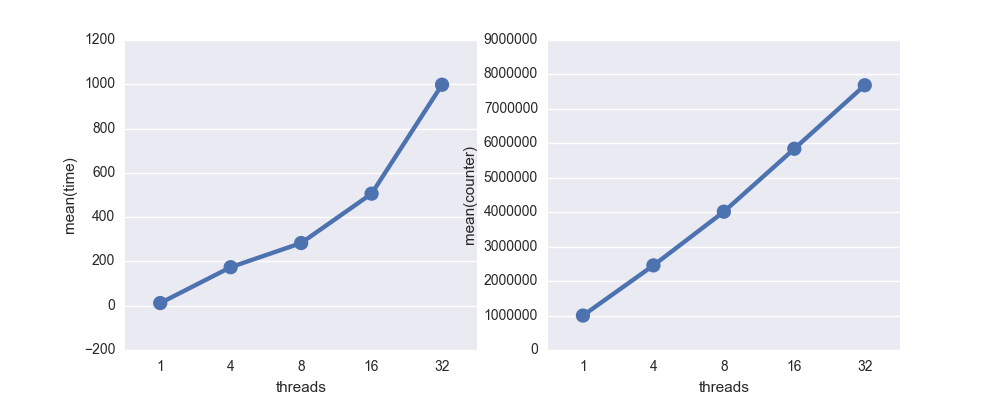
\includegraphics[width=20cm]{Q6_second.png}
\end{figure}
\section*{Q7}
\begin{figure}[h]
	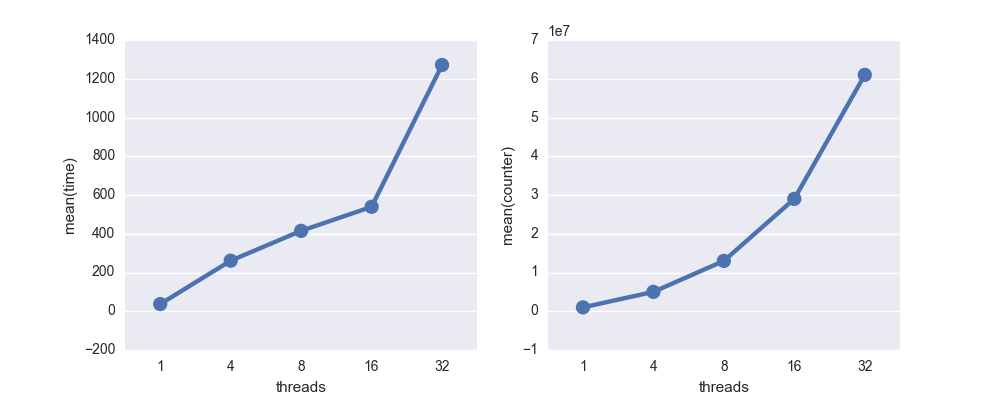
\includegraphics[width=20cm]{Q7.png}
\end{figure}
First, we see that the counter was locked appropriately: its value is the correct value as expected, in comparison to the previous question.
Now we look at the graph and see that it appears to have non-linear growth. The slowdown is because threads must wait for the lock to be unlocked.
This result was expected because of Amdahl?s Law: Most of our program is not parallelized
\pagebreak
\section*{Q8}
\begin{figure}[h]
	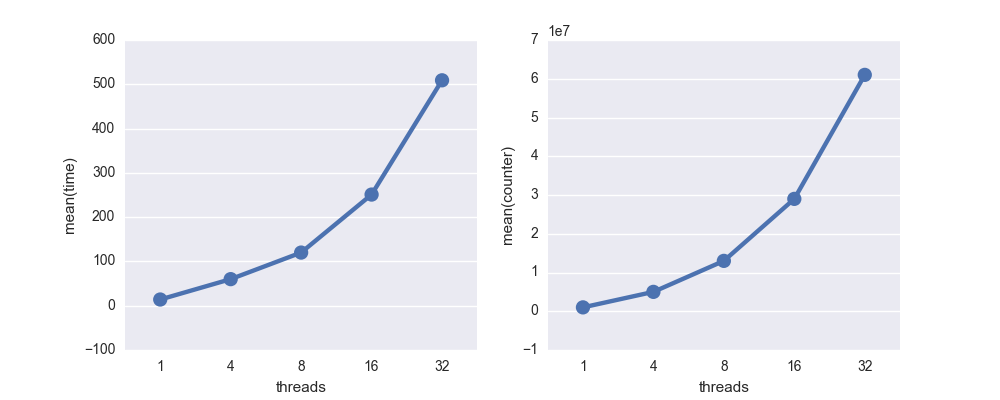
\includegraphics[width=20cm]{Q8_second.png}
\end{figure}
\begin{figure}[h]
	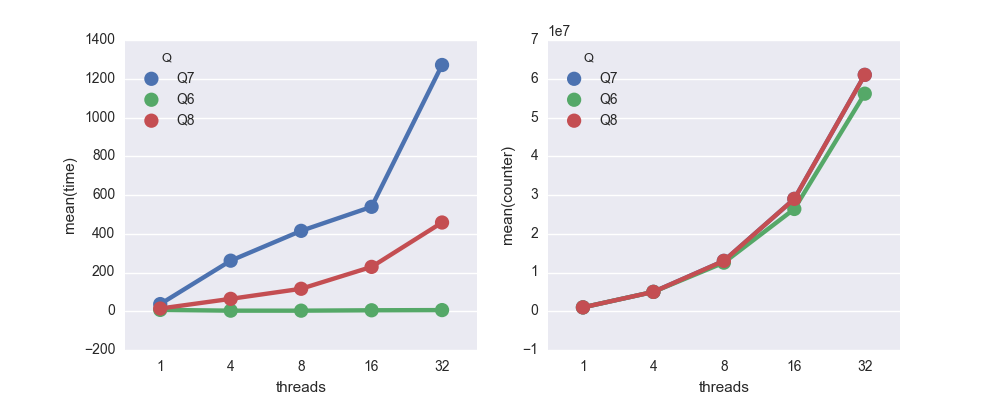
\includegraphics[width=20cm]{Q8_2_second.png}
\end{figure}
On the bottom right plot, question 7's line is masked by question 8's line since the counter values are the same.


\end{enumerate}



\end{document}
